\documentclass[12pt]{article}

\usepackage[margin=1in]{geometry}
\geometry{lettersize}

\usepackage{graphicx}
\usepackage{float}
\usepackage{wrapfig}
\usepackage{caption}
\usepackage{subcaption}

\linespread{1.2}

\renewcommand{\maketitle}{
    \begin{flushright}
        {\LARGE \textbf{Randomization in Path Planning}}


    {\large \textsc{Wenhan Zhu (Cosmos)} \\ \textit{University of Waterloo}}
    \\ \today

    \end{flushright}
}

\begin{document}

\maketitle

\section*{Introduction}
Many path planning algorithms rely on randomness for fast calculation. In many situations, calculating the optimal path is not feasible or time consuming. So many algorithms focuses generating a path quickly and improves the path if time allows. Rapidly-exploring random tree (RRT)\cite{LaValle1998} is one of these algorithms. This report discusses what is RRT and it's comparison to another popular path planning algorithm Probabilistic Roadmap (PRM) \cite{Kavraki1996}. And at last focuses on the improvements on RRT and some open ideas on the topic.

\section*{Motivation}
My previous research focuses on path planning for autonomous vehicles. In particular the path planning in the local planner. The local planner plans the exact vehicle path to navigate on the road. It generates an exact path that the vehicle needs to follow and a corresponding speed profile that guides the controller. As part of the autonomous driving software it needs to run be updates in very short intervals and requires the path to be executable by the vehicle. Many research has been conducted in this area, but there are still no dominating solution when the scenario is complex. This is mainly due to dynamic objects and the unpredictable behaviours of human operated vehicles on the road. I've come across RRT when I was studying animations and AI in games. It turns out that RRT was originally designed to solve the problem of motion planning for robotics. Which is highly related to the field of autonomous vehicles. However, many other problem still remain unsolved for such approach. More details are discussed in the later sections of this report.

\section*{PRM and RRT}
Both PRM and RRT are introduced in the late 90s to solve the problem of having a continuous state space and obstacles that needs to be avoided, how to generate a path between a start state and end state in the state spaces. Many applications of both the algorithms and it's variant are used in path planning. A brief overview of both the algorithms are discussed in the following sections. 

\begin{figure}
\centering
\begin{subfigure}{.5\textwidth}
    \centering
    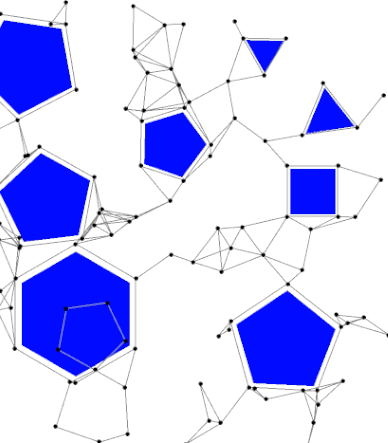
\includegraphics[width=.6\linewidth]{prm-example.png}
    \caption{PRM example (Source: Wiki)}
    \label{fig:prm}
\end{minipage}%
\begin{subfigure}{.5\textwidth}
    \centering
    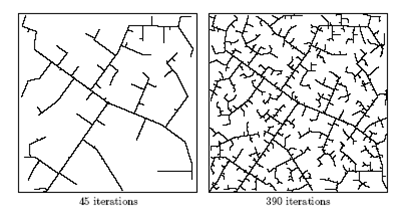
\includegraphics[width=.6\linewidth]{rrt-example.png}
    \caption{RRT example (Source: Wiki)}
    \label{fig:rrt}
\end{minipage}
\end{figure}



\subsection*{PRM}
In principle, PRM creates a set of points as a boundary for each obstacle in the space. Then it adds random points in the space and connects points that are with in a range and does not cross over obstacles. After adding many points so that the graph is connected, we can then use search algorithms such as A* on the graph to achieve the shortest path.

\subsection*{RRT}
As its name, RRT expands a tree with a root at the starting state and randomly sample from the space and connect the sample to the closest node on the existing tree if a feasible connection can be found. Once we are able to connect the goal to the tree, we can back track the nodes of the tree from where it was connected to the root. 

\subsection*{Comparison}



\bibliographystyle{alpha}

\bibliography{sample}

\end{document}
